\documentclass[border=10pt]{standalone}
\usepackage{tikz}\usepackage{amsmath}\usetikzlibrary{arrows.meta}
\begin{document}
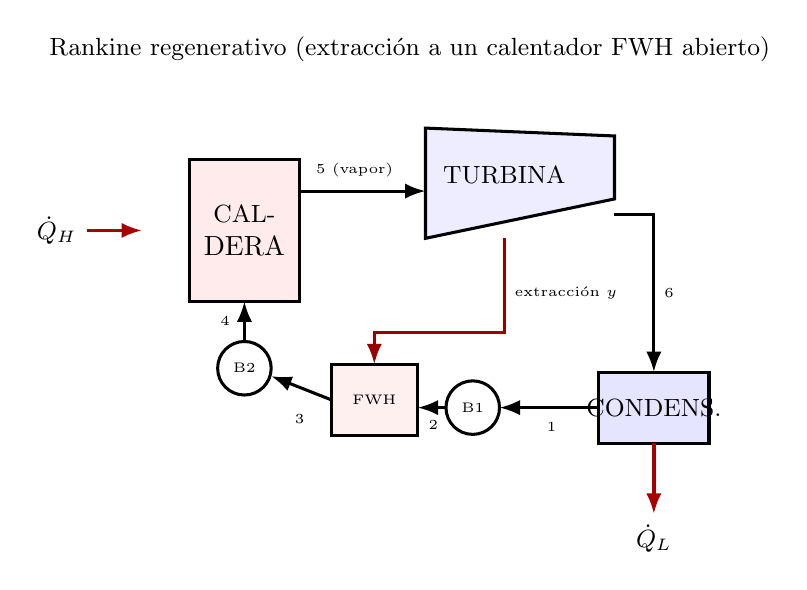
\begin{tikzpicture}[line width=1pt,>={Latex[length=2.6mm]}]
  % caldera
  \fill[red!8] (0,1.8) rectangle (1.4,3.6); \draw[line width=1.1pt] (0,1.8) rectangle (1.4,3.6);
  \node[align=center] at (0.7,2.7){\small CAL-\\DERA};
  % turbina (con extraccion)
  \fill[blue!7] (3.0,2.6)--(5.4,3.1)--(5.4,3.9)--(3.0,4.0)--cycle; \draw[line width=1.1pt] (3.0,2.6)--(5.4,3.1)--(5.4,3.9)--(3.0,4.0)--cycle;
  \node at (4.0,3.4){\small TURBINA};
  % condensador
  \fill[blue!10] (5.2,0) rectangle (6.6,0.9); \draw[line width=1.1pt] (5.2,0) rectangle (6.6,0.9);
  \node at (5.9,0.45){\small CONDENS.};
  % bomba 1 (cond->FWH) y bomba 2 (FWH->caldera)
  \draw[line width=1.1pt] (3.6,0.45) circle (0.34); \node at (3.6,0.45){\tiny B1};
  \draw[line width=1.1pt] (0.7,0.95) circle (0.34); \node at (0.7,0.95){\tiny B2};
  % calentador de agua de alimentacion (FWH abierto)
  \fill[red!6] (1.8,0.1) rectangle (2.9,1.0); \draw[line width=1.1pt] (1.8,0.1) rectangle (2.9,1.0);
  \node[align=center] at (2.35,0.55){\tiny FWH};
  % flujos principales
  \draw[->,line width=1.1pt] (1.4,3.2)--(3.0,3.2); \node[above] at (2.1,3.25){\tiny 5 (vapor)};
  \draw[->,line width=1.1pt] (5.4,2.9)--(5.9,2.9)--(5.9,0.9); \node[right] at (5.9,1.9){\tiny 6};
  \draw[->,line width=1.1pt] (5.2,0.45)--(3.94,0.45); \node[below] at (4.6,0.4){\tiny 1};
  \draw[->,line width=1.1pt] (3.26,0.45)--(2.9,0.45); \node[below] at (3.1,0.42){\tiny 2};
  \draw[->,line width=1.1pt] (1.8,0.55)--(1.04,0.85); \node[below] at (1.4,0.5){\tiny 3};
  \draw[->,line width=1.1pt] (0.7,1.29)--(0.7,1.8); \node[left] at (0.65,1.55){\tiny 4};
  % extraccion de la turbina al FWH
  \draw[->,red!60!black,line width=1.2pt] (4.0,2.6)--(4.0,1.4)--(2.35,1.4)--(2.35,1.0); \node[right] at (4.0,1.9){\tiny extracción $y$};
  % interacciones
  \draw[<-,red!65!black,line width=1.2pt] (-0.6,2.7)--(-1.3,2.7); \node[left] at (-1.3,2.7){\small $\dot Q_H$};
  \draw[->,red!65!black,line width=1.2pt] (5.9,0)--(5.9,-0.9); \node[below] at (5.9,-0.9){\small $\dot Q_L$};
  \node at (2.8,5.0){\small Rankine regenerativo (extracción a un calentador FWH abierto)};
\end{tikzpicture}
\end{document}
